\documentclass[a4paper,12px]{article}
\usepackage{graphicx}
\usepackage[english]{babel}
\usepackage{fullpage}
\usepackage{xfrac}
\usepackage{fancyhdr}
\usepackage{lastpage}
\usepackage{xifthen}
\usepackage[linesnumberedhidden, titlenotnumbered]{algorithm2e}
\usepackage{lipsum}
\usepackage{hyperref}
\usepackage{array}
\usepackage{tabularx}
\usepackage{caption}
\usepackage{amsfonts}
\usepackage{amssymb}
\usepackage{amsmath}
\usepackage{mathtools}
\usepackage{placeins}
\usepackage{enumitem}
\usepackage[noabbrev]{cleveref}
\usepackage[utf8]{inputenc}
\usepackage{multirow}

\usepackage{minted}
\usepackage{listings}
\usepackage{dsfont}
\usepackage{units}

\pagestyle{fancy}
\lhead{
\includegraphics[width=7cm]{logoUvA}}
\rhead{\footnotesize \textsc {Report\\ \opdracht}}
\lfoot%
{%
    \footnotesize \studentA%
    \ifthenelse{\isundefined{\studentB}}{}{\\ \studentB}
    \ifthenelse{\isundefined{\studentC}}{}{\\ \studentC}
    \ifthenelse{\isundefined{\studentD}}{}{\\ \studentD}
    \ifthenelse{\isundefined{\studentE}}{}{\\ \studentE}
}
\cfoot{}
\rfoot{\small \textsc {Page \thepage\ of~\pageref{LastPage}}}
\renewcommand{\footrulewidth}{0.5pt}

\fancypagestyle{firststyle}
{%
    \fancyhf{}
    \renewcommand{\headrulewidth}{0pt}
    \chead{
\includegraphics[width=7cm]{logoUvA}}
    \rfoot{\small \textsc {Page \thepage\ of~\pageref{LastPage}}}
}

\setlength{\topmargin}{-0.3in}
\setlength{\textheight}{630pt}
\setlength{\headsep}{40pt}
\setlength{\parindent}{0pt}

% =================================== DOC INFO ===================================

\newcommand{\opdracht}{Theoretical Excercises}
\newcommand{\titel}{PGLEc MPP}
\newcommand{\docent}{Alban Ponse}
\newcommand{\cursus}{Theoretische aspecten van de Programmatuur}
\newcommand{\vakcode}{}
\newcommand{\datum}{\today}
\newcommand{\studentA}{Maico Timmerman}
\newcommand{\uvanetidA}{10542590}
%\newcommand{\studentB}{Tim van Zalingen}
\newcommand{\uvanetidB}{10784012}
% \newcommand{\studentC}{Boudewijn Braams}
\newcommand{\uvanetidC}{10401040}
% \newcommand{\studentD}{Govert Verkes}
\newcommand{\uvanetidD}{10211748}
%\newcommand{\studentE}{Naam student 5}
\newcommand{\uvanetidE}{UvAnetID student 5}

% ===================================  ===================================

\begin{document}
\thispagestyle{firststyle}
\begin{center}
    \textsc{\Large \opdracht}\\[0.2cm]
    \rule{\linewidth}{0.5pt} \\[0.4cm]
    {\huge \bfseries \titel}
    \rule{\linewidth}{0.5pt} \\[0.2cm]
    {\large \datum\\[0.4cm]}

    \begin{minipage}{0.4\textwidth}
        \begin{flushleft}

            \emph{Student:}\\
            {\studentA\\ {\small \uvanetidA\\[0.2cm]}}
            \ifthenelse{\isundefined{\studentB}}{}{\studentB\\ {\small \uvanetidB\\[0.2cm]}}
        \end{flushleft}
    \end{minipage}~%
    \begin{minipage}{0.4\textwidth}
        \begin{flushright}
            \emph{Lecturer:} \\
            \docent\\[0.2cm]
            \emph{Course:} \\
            \cursus\\[0.2cm]
            % \emph{Student:}\\
            \ifthenelse{\isundefined{\studentC}}{}{\studentC\\ {\small \uvanetidC\\[0.2cm]}}
            \ifthenelse{\isundefined{\studentD}}{}{\studentD\\ {\small \uvanetidD\\[0.2cm]}}
            \ifthenelse{\isundefined{\studentE}}{}{\studentE\\ {\small \uvanetidE\\ [0.2cm]}}
        \end{flushright}
    \end{minipage}\\[1 cm]
\end{center}


% =================================== CONTENTS ===================================

% \tableofcontents

\newcommand{\Sum}[2]{\sum^{#2}_{#1}}
\newcommand{\E}[1]{{\mathbb{E}\left[#1\right]}}
\newcommand{\var}[1]{{\text{var}\left[#1\right]}}
\newcommand{\diffpart}[1]{\frac{\partial}{\partial{} #1}}
\newcommand{\?}{\stackrel{?}{=}}
\newcommand{\intinf}{\int\limits_{-\infty}^{\infty}}
\newcommand{\intnulinf}{\int\limits_{0}^{\infty}}
\newcommand{\intpi}{\int\limits_{0}^{2\pi}}
\newcommand{\argmin}[1]{\underset{#1}{\mathop{\mathrm{argmin}}}}
\newcommand{\argmax}[1]{\underset{#1}{\mathop{\mathrm{argmax}}}}
% =================================== MAIN TEXT ===================================


\section{Creating the formula $(x1+1)\cdot(x2+1)$}

\begin{minted}{C}
setZero;

x=y; succ;

x=y; succ;

//Set the x1 to 2
x1=y;

x=y; succ;

//Set the x2 to 3
x2=y;
\end{minted}

\begin{figure}[h]
    \centering
    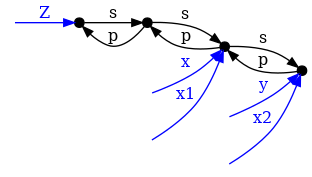
\includegraphics[width=0.8\linewidth]{f1.png}
    \caption{Initial state $x1=2$ and $x2=3$ before the algorithm.}
\end{figure}
\FloatBarrier%

\begin{minted}{C}

// (x1 + 1)
x=x1; succ; x1=y;

// (x2 + 1)
x=x2; succ; x2=y;

\end{minted}

\begin{figure}[h]
    \centering
    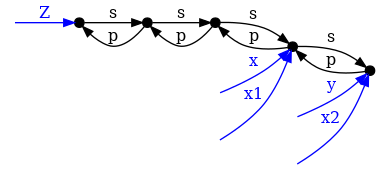
\includegraphics[width=0.8\linewidth]{f2.png}
    \caption{State after calling succ on both $x1$ and $x2$.}
\end{figure}
\FloatBarrier%


\begin{minted}{C}
// init for multiply;
One = Z.s;
x3 = x1;
x4 = x2;
y = x2;

// Start multiply loop;
L1;
-x3==One{;
    //decrement the down-wards counter by 1;
    x3 = x3.p;

    // Set variables of ready for the addition;
    x1 = x4;
    x2 = y;

    add;

    // Loop until x3 is equal to 1;
    ##L1;
}{;
};
\end{minted}
\begin{figure}[h]
    \centering
    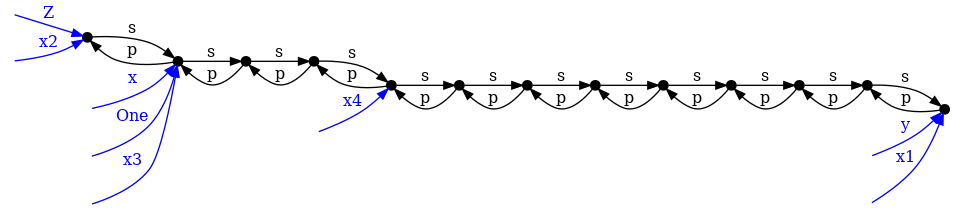
\includegraphics[width=0.8\linewidth]{f3.png}
    \caption{Final state of $(x1+1)\cdot(x2+1)$ with $x1=2$ and $x2=3$}
\end{figure}
\FloatBarrier%

The program will first call the successor function (\verb|succ|) on both $x1$ and $x2$, which means can
never be 0.

Implementation of the algorithm is as following:

$$\begin{displaystyle}
    \forall m,n \in \mathbb{N}:
  \begin{cases}
      m \cdot n = m \cdot 1 & =m\\
      m \cdot (n + 1) &= m \cdot n + m
  \end{cases}
\end{displaystyle}$$

The addition (\verb|add|) in the program is the one provided, defined as:

$$\begin{displaystyle}
    \forall m,n \in \mathbb{N}:
  \begin{cases}
      m + n  = m + 0 &=m \\
      m + n  &=(m+1) + (n-1)
  \end{cases}
\end{displaystyle}$$




% =================================== REFERENCES ===================================

% \clearpage

% \bibliographystyle{apalike}
% \bibliography{report}

\end{document}
